\section{Irreduzibilitatskriterien}

Sei $R$ ein faktorieller Ring, $K = \Quot(R)$.

\begin{remark}
	Sei $f \in K[x]$. Wir suchen hinreichende Kriterien dafür, dass $f \in K[x]$ irreduzibel ist.
	\begin{enumerate}[label=(\alph*)]
		\item Ist $c \in K^{\times}$ so gilt: $f$ ist irreduzibel $\Longrightarrow c \cdot f$ ist irreduzibel. Wir können also z.B. ohne Einschränkung annehmen, dass $f$ normiert ist.
		\item $\deg(f) = 1$: $f$ ist irreduzibel und hat Nullstellen in $K$.
		\item $\deg(f) \ge 2$: $f$ hat Nullstellen in $K \Rightarrow f$ reduzibel, da $f(a) = 0 \Rightarrow f(x) = (x-a)\cdot g(x)$, $\deg(g) = \deg(f) - 1 > 0$
		\item $\deg(f) \le 3$: $f$ hat keine Nullstelle in $K \Rightarrow f$ ist irreduzibel, da $f=gh$, $gh \not \in K^{\times}\Rightarrow \deg(g) = 1$ oder $\deg(h) = 1$\\
		\textbf{Achtung}: Für $\deg(f) \ge 4$ ist dies im Allgemeinen falsch! Zum Beispiel $f = x^4 + 2x^2 + 1 = (x^2 +1)^2 \in \ratio[x]$
	\end{enumerate}
\end{remark}

\begin{proposition}[\person{Eisenstein}'sches Irreduzibilitätskriterium]
	\proplbl{2_7_2}
	Sei $f = \sum_{i=0}^{n} a_i x^i \in R[x]\setminus R$ primitiv, und $p \in R$ prim mit $p\nmid a_n$, $p \mid a_i$ für $i = 0, \dots,n-1$, $p^2 \nmid a_0$. Dann ist $f$ irreduzibel in $R[x]$ und somit auch in $K[x]$.
\end{proposition}

\begin{proof}
	Sei $f=g\cdot h$ mit $g=\sum_{i=0}^k b_ix^i$, $h=\sum_{i=0}^l c_ix^i\in R[x]$ und $n=k+l$.
	\begin{itemize}
		\item $p\nmid a_n = b_k\cdot c_l\Rightarrow p\nmid b_k$ und $p\nmid c_l$
		\item $p\mid a_0 = b_0\cdot c_0$ und $p^2\mid a_0\Rightarrow$ ohne Einschränkung $p\mid b_0$, aber $p\nmid c_0$
	\end{itemize}
	Sei $m=\max\{i\in\natur\mid p\mid b_0,...,p\mid b_i\}\in \{0,...,k-1\}$ \\
	$\Rightarrow a_{m+1} = \underbrace{b_0c_{m+1}+b_1c_m+...+b_mc_1}_{=0\mod p} + \underbrace{b_{m+1}c_0}_{\neq 0\mod p}$ \\
	$\Rightarrow p\nmid a_{m+1}$ \\
	$\Rightarrow m+1\ge n\Rightarrow k\ge m+1\ge n = k+l\Rightarrow k=n$ und $l=0$ \\
	$\Rightarrow h\in R\xRightarrow{f\text{ primitiv}} h\in R^\times \subseteq R[x]^\times$ \\
	Somit ist $f$ irreduzibel in $R[x]$ und mit \propref{2_6_10} und $f\notin R$ folgt, dass $f$ irreduzibel in $K[x]$ ist.
\end{proof}

\begin{example}
	Ist $p \in R$ prim, $n > 0$ ist $f = X^n-p$ nach \propref{2_7_2} irreduzibel in $K[x]$
	\begin{enumerate}[label=(\alph*)]
		\item $R = \whole$: $x^2 -5$, $x^7 - 3$ irreduzibel in $\ratio[x]$
		\item $R = F[t]$, $F$ Körper: $x^2-t$, $x^5 + t +1$ irreduzibel in $F[t][x] = F[t,x]$
	\end{enumerate}
\end{example}

\begin{proposition}[Reduktionskriterium]
	Sei $0 \neq f = \sum_{i=0}^{n} a_i x^i \in R[x]\setminus R$ und $p \in R$ prim mit $p \nmid a_n$. Ist $\bar{f} \in \left(\lnkset{R}{(p)} \right)[x]$ irreduzibel, so auch $f$ irreduzibel in $K[x]$.
\end{proposition}
\begin{proof}
	Schreibe $f=c\cdot f_0$, $c\in R$ und $f_0\in R[x]$ primitiv. Wenn $p\nmid a_n$, dann folgt $p\nmid c$ und $p\nmid \LC(f_0)$. Sei also ohne Einschränkung $f=f_0$ primitiv. Sei $f=g\cdot h$ mit $g=\sum_{i =0}^k b_ix^i$, $h=\sum_{i =0}^l c_ix^i\in R[x]$ und $k+l=n$. Wenn $p\nmid a_n$, dann $p\nmid b_k$ und $p\nmid c_l$. \\
	$\Rightarrow\bar{f} = \bar{g}\cdot\bar{h}$, wobei $\deg(\bar{f})=n$, $\deg(\bar{g})=k$ und $\deg(\bar{h})=l$ \\
	$\xRightarrow{\bar{f}\text{ irreduzibel}}$ ohne Einschränkung $\bar{g}\in\left(\lnkset{R}{(p)}\right)[x]^\times$, insbesondere $k=0\Rightarrow l=n$ \\
	$\Rightarrow g\in R\xRightarrow{f\text{ primitiv}} g\in R^\times$ \\
	$\Rightarrow f$ irreduzibel in $K[x]$
\end{proof}

\begin{example}
	$R=\whole$: $f=x^3+3x^2+2x+1$ ist irreduzibel in $\ratio[x]$, denn
	\begin{align}
		\bar{f} = x^3+x^2+1\in \mathbb{F}_2[x]\notag
	\end{align}
	hat keine Nullstellen in $\mathbb{F}_2=\{0,1\}$.
\end{example}

\begin{remark}
	Die Nullstellen von $x^n-1$ in $\comp$, also die $n$-Torsion $\comp^\times[n]$ von $\comp^\times$ nennt man die $n$-ten \begriff{Einheitswurzeln}. Diesel bilden eine zyklische Gruppe der Ordnung $n$, erzeugt von $\zeta_n = e^{\frac{2\pi i}{n}}$. Elemente von $\comp^\times$ der Ordnung genau $n$ nennt man \begriff[Eineheitswurzeln!]{primitive $n$-te Einheitswurzel}.
	
	\begin{center}
		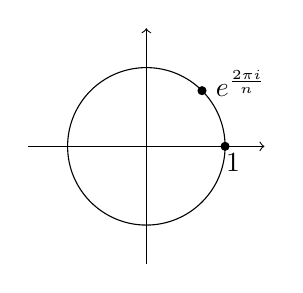
\begin{tikzpicture}
			\draw[->] (-1.5,0) --(1.5,0);
			\draw[->] (0,-1.5) -- (0,1.5);
			\draw (0,0) circle (1);
			\draw[fill=black] (0.707,0.707) circle (0.05);
			\node at (1.2,0.8) (a) {$e^{\frac{2\pi i}{n}}$};
			\draw[fill=black] (1,0) circle (0.05);
			\node at (1.1,-0.2) (b) {1};
		\end{tikzpicture}
	\end{center}
\end{remark}

\begin{definition}[$p$-tes Kreisteilungspolynom]
	Für $p\in\natur$ prim ist
	\begin{align}
		\Phi_p = \frac{x^p-1}{x-1} = x^{p-1} + x^{p-2} + ... + x + 1\in\whole[x]\notag
	\end{align}
	das $p$-te \begriff{Kreisteilungspolynom}.
\end{definition}

\begin{remark}
	Die Nullstellen von $\Phi_p$ sind genau die primitiven Einheitswurzeln:
	\begin{align}
		\Phi_p = \prod_{k=1}^{p-1} (x-\zeta_p^k)\notag
	\end{align}
\end{remark}

\begin{proposition}
	Für $p\in\natur$ prim ist $\Phi_p$ irreduzibel in $\ratio[x]$.
\end{proposition}
\begin{proof}
	Das Polynom $\Phi_p(x+1)$ ist ein Eisensteinpolynom zur Primzahl $p$, also irreduzibel nach \propref{2_6_2}. Da $f(x)\mapsto f(x+1)$ ein Automorphismus von $\ratio[x]$ ist, ist damit auch $\Phi_p(x)$ irreduzibel.
\end{proof}

\begin{example}
	\proplbl{2_7_10}
	Sei $f=2x^7-100\in \ratio[x]\Rightarrow$ Multiplikation mit Einheit $2^{-1}\Rightarrow x^7-50\Rightarrow$ \person{Eisenstein}. \\
	\textbf{Achtung:} $2x^7-100\in\real[x]$ ist nicht irreduzibel!
\end{example}

\begin{*anmerkung}
	In \propref{2_7_10} ist \person{Eisenstein} im ersten Schritt nicht anwendbar, da $2\mid 100$, aber auch $2\mid \LC(f)=2$ und $5\mid 100$, aber auch $5\mid 100^2$.
\end{*anmerkung}